\section{Results}
\label{sec:results}

The sweep completed 5{,}520 runs with \textbf{28 failures (0.51\%)}, all from
a single cause: two cells in which no choice of five path edges could be
closed without disconnecting the origin--destination pair. That is the
fragility result of Section~\ref{sec:fragility}, not a defect. All
invariants hold on the real data: stretch, post-disruption stretch, and both
walk-only stretch columns are $\geq 1.0$ with zero violations.

\subsection{Extraction provenance decides what a Physarum number means}
\label{sec:provenance}

We begin here because every later Physarum figure depends on it.

Pooled across extraction methods, Physarum matches the optimal route on
\textbf{90.0\%} of undisrupted pairs at heavy demand and 86.7\% at light ---
reproducing the accuracy the literature reports for this model. Restricted to
its own maximum-flux walk, the same solves give \textbf{23.3\% and 16.7\%}.
The walk produces any path at all on 69.8\% of Physarum rows.

Table~\ref{tab:provenance} shows why pooling destroys the distinction.

\begin{table}[t]
\caption{Provenance of Physarum's reported path, over all 776 successful
Physarum rows. The median stretch is 1.000 in \emph{every} class.}
\label{tab:provenance}
\centering
\begin{tabular}{lrrrr}
\toprule
Extraction method & Own? & $n$ & Share & Exact \\
\midrule
\texttt{full\_graph\_fallback}     & no  & 315 & 40.6\% & 95.2\% \\
\texttt{max\_flux\_walk}           & yes & 232 & 29.9\% & 74.6\% \\
\texttt{theta\_subgraph\_fallback} & no  & 229 & 29.5\% & 94.3\% \\
\bottomrule
\end{tabular}
\end{table}

\textbf{About 70\% of Physarum's reported paths did not come from its own
extraction}, and \texttt{full\_graph\_fallback} is plain Dijkstra. Because
the median stretch is exactly 1.000 within each class, a pooled median cannot
separate ``the model found the optimum'' from ``the fallback returned
Dijkstra's answer''. A pooled Physarum-versus-Dijkstra comparison is
therefore partly circular.

The effect is sharper still on recovery, and it is \emph{mode-dependent} in a
way a pooled table conceals:

\begin{center}
\begin{tabular}{lrrr}
\toprule
Start mode & Walk & Threshold & Full-graph (Dijkstra) \\
\midrule
Cold & 95  & 201 & 62 \ \ (17.3\%) \\
Warm & 119 & \textbf{0} & \textbf{239 \ (66.8\%)} \\
\bottomrule
\end{tabular}
\end{center}

With roughly 98.8\% of retained tubes below $\theta$, warm start's threshold
subgraph never connects the pair --- a hard zero across all 358 warm cells
--- so \textbf{warm Physarum reports plain Dijkstra's path on two-thirds of
all recoveries}. The two start modes reach an answer by different routes, and
only one of them involves the model.

Fig.~\ref{fig:convergence} is the clearest single piece of evidence: in two
of three panels the with-fallback curve sits at stretch 1.0 from iteration
one, because it was Dijkstra's answer before the model did any work.

\begin{figure}[t]
\centering
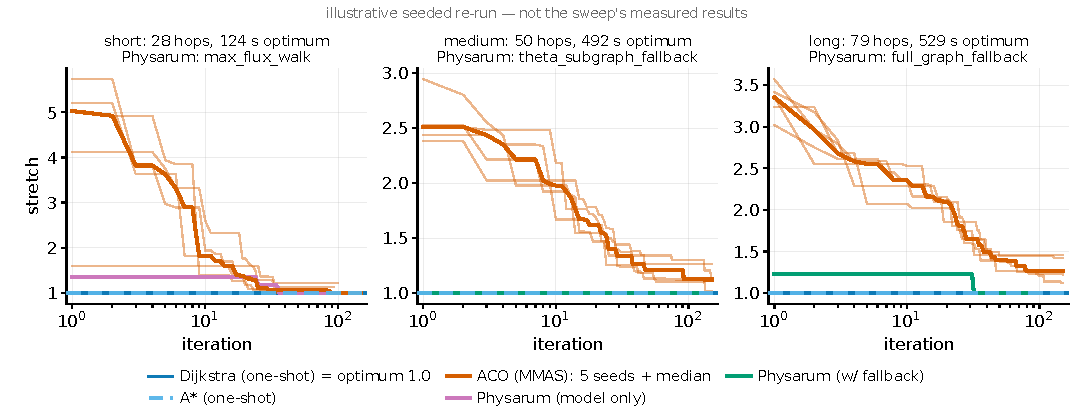
\includegraphics[width=\columnwidth]{fig01_convergence.pdf}
\caption{Cost versus iteration across three distance strata. The Physarum
with-fallback series begins at stretch 1.0 in two of three panels: that is
the fallback, not convergence.}
\label{fig:convergence}
\end{figure}

We therefore report Physarum as two labelled series everywhere below, and
never pool them.

\subsection{Pre-disruption path quality}

Table~\ref{tab:quality} gives the undisrupted comparison. Dijkstra and A*
are exact by construction, and their agreement is the admissibility check of
Section~\ref{sec:algorithms} rather than a result.

\begin{table}[t]
\caption{Pre-disruption path quality, deduplicated on the initial solve.
95\% CIs from the clustered bootstrap.}
\label{tab:quality}
\centering
\small
\begin{tabular}{llrrrr}
\toprule
Series & Traffic & $n$ & Median & Exact & $\leq$10\% \\
\midrule
Dijkstra / A*      & all   & 60  & 1.0000 & 100\%  & 100\% \\
\midrule
ACO (MMAS)         & light & 150 & 1.0052 & 43.3\% & 81.3\% \\
ACO (MMAS)         & heavy & 150 & 1.0209 & 44.0\% & 58.0\% \\
\midrule
Physarum, pooled   & light & 30  & 1.0000 & 86.7\% & 93.3\% \\
Physarum, pooled   & heavy & 30  & 1.0000 & 90.0\% & 93.3\% \\
Physarum, model only & light & 30 & 1.0849 & 16.7\% & 36.7\% \\
Physarum, model only & heavy & 30 & 1.1007 & 23.3\% & 33.3\% \\
\bottomrule
\end{tabular}
\end{table}

ACO's exact-match share is 43--44\% with median stretch 1.005 (light) and
1.021 (heavy). Its per-seed within-10\% spread is tight (0.767--0.833 light,
0.567--0.633 heavy), so this is not a seed artefact. We note separately that
ACO \emph{misses} the exit criterion we set for it in advance --- stretch
$\leq 1.10$ on $\geq 90\%$ of pairs --- reaching 73.3\% under free flow
(95\% CI [58.7, 86.7], the whole interval below the bar) and 80.7\% under
BPR heavy on a held-out pair draw. The failure mode is a colony settling on a
badly wrong corridor and never leaving it: MMAS's own convergence criterion
fires on 79\%/69\% of those solves, so they are settled local optima rather
than unfinished searches. We report this rather than retuning until it
passes.

\subsection{Recovery: warm start buys speed and charges quality}
\label{sec:recovery}

\begin{table}[t]
\caption{Recovery cost, scenarios S1--S6.}
\label{tab:recovery}
\centering
\small
\begin{tabular}{llrrrr}
\toprule
Algorithm & Start & $n$ & Iters & Wall (s) & 1 iter \\
\midrule
Dijkstra  & cold & 358 & 1.0  & 0.031 & 100\% \\
A*        & cold & 358 & 1.0  & 0.027 & 100\% \\
ACO       & warm & 1790 & 69.0 & 34.07 & 0\% \\
ACO       & cold & 1790 & 110.0 & 59.80 & 0\% \\
Physarum  & warm & 358 & 42.0 & 0.235 & \textbf{48.3\%} \\
Physarum  & cold & 358 & 98.0 & 5.661 & 0\% \\
\bottomrule
\end{tabular}
\end{table}

\begin{figure}[t]
\centering
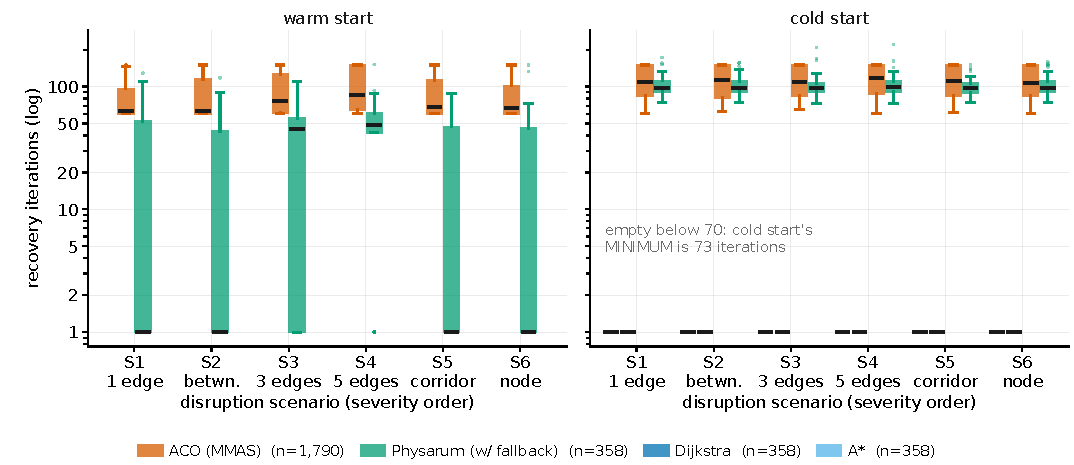
\includegraphics[width=\columnwidth]{fig02_recovery_by_scenario.pdf}
\caption{Recovery iterations by closure severity. Dijkstra and A* collapse to
a line at one iteration. S0 is absent by construction: it has no recovery to
measure, and plotting its nulls as zeros would fabricate a measurement. The
warm panel omits the classical routers, which have no warm mode.}
\label{fig:byscenario}
\end{figure}

\textbf{Dijkstra wins on wall-clock and we report it plainly.} A recompute on
this graph costs about 31\,ms; the bio-inspired methods take seconds. The
interesting quantities are iterations-to-adapt and post-disruption quality.

Paired on identical cells, warm start reduces Physarum's recovery by
\textbf{2.97$\times$ in iterations} (warm faster on 350 of 358,
$p=3.2\times10^{-59}$) and \textbf{6.87$\times$ in wall-clock} (336 of 358,
$p=9.0\times10^{-52}$). For ACO the gains are smaller but significant:
1.26$\times$ and 1.56$\times$ ($n=1{,}790$, $p=1.5\times10^{-184}$).

Two observations matter more than the ratios. First, \textbf{the
distribution is bimodal, not merely shifted}: 48.3\% of warm recoveries
converge in exactly one iteration, while cold start never does and its
minimum is 73 (Fig.~\ref{fig:warmcold}). The retained field already encodes a
viable detour, so a single adaptation step suffices. The ratio of the two
medians is not a valid statistic here, and an earlier version of this
analysis that computed one produced a spurious 24$\times$.

Second, \textbf{per-iteration cost is essentially identical} warm versus cold
(0.0511 versus 0.0538\,s), which is what establishes that the saving is
fewer iterations rather than cheaper ones --- the precise claim the
self-healing framing makes.

\begin{figure}[t]
\centering
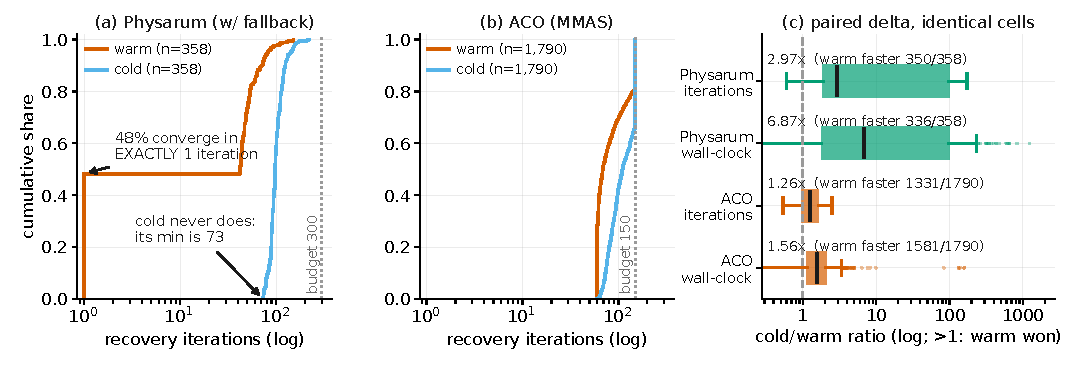
\includegraphics[width=\columnwidth]{fig07_warm_vs_cold.pdf}
\caption{Warm versus cold recovery. The bimodality --- a mode at exactly one
iteration and another near 50 --- is the shape of the result, and is why we
report paired ratios rather than a ratio of medians.}
\label{fig:warmcold}
\end{figure}

\subsubsection{What warm start costs}

Warm start is \emph{not} free, and the cost appears in two places.

On the \textbf{reported path}, paired across all 358 recovery cells, cold
start is better: cold wins on 57 cells, warm on 11, with 290 ties
($p=4.3\times10^{-7}$; mean 1.0669 versus 1.0311, exact match 282 versus
315). On the \textbf{model's own extraction}, the warm maximum-flux walk
completes a path on only 36.3\% of recoveries against cold's 59.5\%.

\begin{figure}[t]
\centering
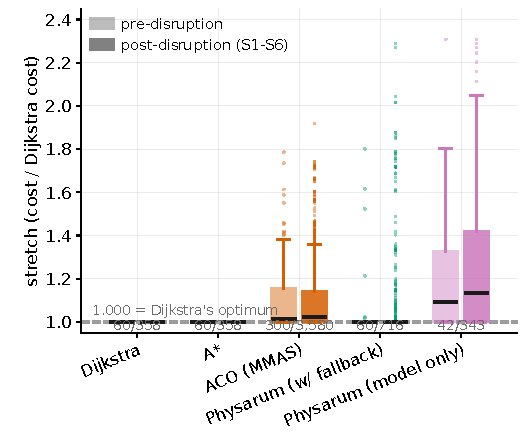
\includegraphics[width=\columnwidth]{fig03_stretch_pre_post.pdf}
\caption{Path quality before and after a closure. Counts beneath each pair are
$n$(pre)\,/\,$n$(post). The two Physarum series are never pooled: the
model-only series is null --- not zero --- on runs where the walk never
completed a path, so its $n$ is smaller by construction.}
\label{fig:prepost}
\end{figure}

An earlier version of this analysis compared the walk's quality unpaired,
across samples of different size, and reported the opposite sign. On the 126
cells where both complete, cold's walk appeared marginally better (1.0127
versus 1.0587, $p=2.7\times10^{-4}$) --- but Section~\ref{sec:adaptation}
shows that this advantage is bought at iteration one by a field that has not
yet run the model, and that at the final iteration the two modes are
statistically indistinguishable.

\subsubsection{Why warm start hurts the walk}

We tested the obvious explanation --- that a retained field keeps driving
flux down now-severed corridors --- and \textbf{refuted it}. A placebo
closure placed at least eight hops from every node of the retained corridor
reproduces almost the entire deficit (warm 43.3\% versus cold 70.0\%,
$n=60$, $p=3.1\times10^{-5}$), and placebo versus a closure sitting directly
on the route is \emph{indistinguishable} (43.3\% versus 41.7\%, $n=60$
paired, $p=1.00$). Spatial locality is flat: the warm walk's terminal node
lies a median 12 hops from the nearest closed edge, and so does cold's
($p=0.356$).

A second candidate --- that warm start simply leaves less conductivity ---
is \emph{analytically impossible}. Scaling $D$ by $c$ scales $w = D/L$ by $c$
and hence $p$ by $1/c$, leaving $Q = w\,\Delta p$ exactly unchanged. We
verified this numerically: rescaling by $10^{-3}$ and $10^{3}$ changes the
flux by less than $10^{-15}$. Only the \emph{shape} of the field can matter,
never its level.

What the data support is this: \textbf{the maximum-flux walk works on a
near-uniform field and stops working as the field converges onto a thin
corridor.} Whether the walk completes on the final pre-disruption iteration,
with the graph fully intact, predicts warm recovery completion on 314 of 358
cells (87.7\%, Fisher $p=1.4\times10^{-50}$). Convergence alone, with no
closure anywhere, drops completion from 69.8\% to 43.0\%. Cold start's
advantage is not that it explores more freely relative to the closure --- it
is that it \emph{rewinds the field to the uniform state the walk can
traverse}.

\begin{figure}[t]
\centering
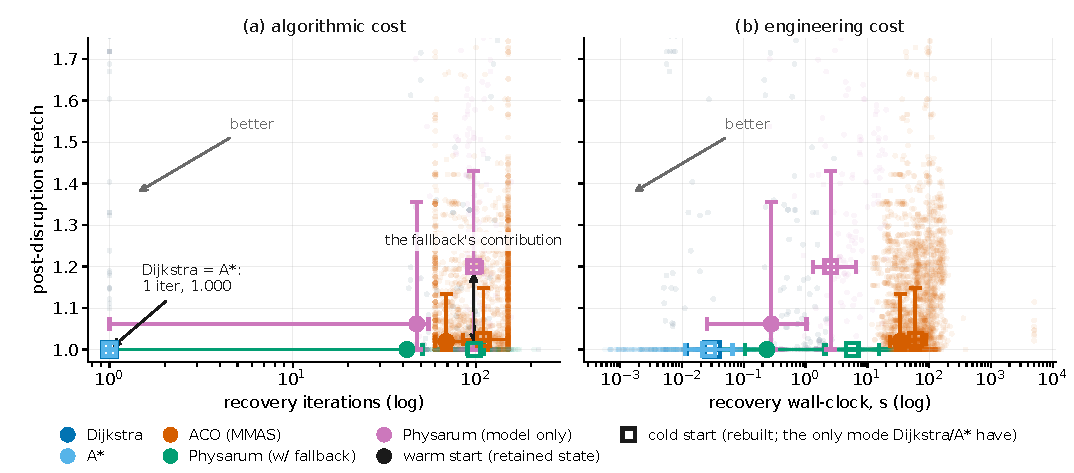
\includegraphics[width=\columnwidth]{fig04_pareto_recovery_vs_quality.pdf}
\caption{The speed-versus-quality trade, and the direct answer to the
question this paper asks. One marker per series and start mode at the median,
with IQR arms on both axes, over a scatter of individual S1--S6 recovery
runs. Dijkstra and A* anchor the lower left: exact paths in one iteration and
roughly 30\,ms. The model-only Physarum series uses the same runs as the
pooled one, so its $x$ is identical and only its $y$ differs --- \emph{the
vertical gap between the two Physarum markers is the fallback's
contribution}.}
\label{fig:pareto}
\end{figure}

\subsection{What adaptation actually contributes}
\label{sec:adaptation}

The preceding result invites the conclusion that convergence is a liability
and that the model should stop earlier. We tested that directly against a
zero-adaptation control: the same pressure solve on a uniform conductivity
field, which is an electrical flow on a travel-time-resistive network
containing none of the Tero dynamics. The control is exact by construction,
since the solver computes pressures and extracts before updating $D$, so its
first iteration \emph{is} the unadapted field.

\begin{table}[t]
\caption{Zero-adaptation control versus the converged field, 60 undisrupted
solves.}
\label{tab:adaptation}
\centering
\begin{tabular}{lrr}
\toprule
 & Uniform (no adaptation) & Converged \\
\midrule
Walk completes      & \textbf{0.567} & 0.433 \\
Walk stretch, median & 1.4367 & \textbf{1.0059} \\
Exact $\mid$ completion & 5.9\% & \textbf{46.2\%} \\
\bottomrule
\end{tabular}
\end{table}

\textbf{Completion and quality move in opposite directions.} The unadapted
field reaches the target more often and produces routes more than 40\% above
optimal; the converged field reaches it less often and is near-optimal when
it does. Paired on the same solves, the unadapted field loses 26--0 to the
best adapted iteration ($n=34$, $p=8.3\times10^{-6}$) and 15--3 to the final
iteration ($n=21$, $p=0.0156$); this reproduces at scale on cold recovery
(120--1, $n=176$, $p=3.2\times10^{-21}$) and warm (27--5, $n=82$,
$p=1.0\times10^{-3}$).

The mechanism is that a near-uniform field is walkable \emph{because} it is
uninformative: flux spreads across many routes, so almost every node has a
positive-flux successor, and the route strung together is poor. This also
resolves the apparent conflict with~\cite{wang2021transition}: their claim
that the dominant path at convergence is the shortest path is about quality,
and on our substrate quality indeed improves with convergence --- what fails
is \emph{completion}, which a complete graph cannot exhibit.

\textbf{No earlier stopping rule is worth adopting.} No fixed iteration count
beats the $\max|\Delta D| < \epsilon$ criterion in any of our three
censuses. A perfect per-cell oracle buys \emph{zero} additional exact
matches, because every exact-match walk is already exact at the final
iteration; it adds only 16 completions of mediocre paths (median stretch
1.2479, none optimal), moving the within-10\% rate from 0.267 to 0.350.
Moreover the walk's best iteration is dispersed (median 26.5, IQR
12.25--33.5), so no fixed rule could capture it, and the router already
retains the best walk across all iterations --- so there is nothing to gain
by stopping at all.

\subsection{The congestion model determines the sign of the effect}

On the undisrupted solve, ACO's within-10\% rate is 81.3\% under light SUMO
demand and 58.0\% under heavy, and paired on the same (OD, seed) cells heavy
is significantly worse ($p=0.036$; 37 pairs pass only under light against 2
only under heavy).

This \emph{reverses} what we measured on the analytic BPR provider, where
congestion improved ACO's outcomes because it flattens the cost surface and
more routes land within 10\% of optimal. The algorithm, the network and the
OD pairs are identical; only the congestion source differs.

\textbf{The sign of the congestion effect is therefore a property of the
congestion model, not of the algorithm}, which is direct evidence for the
bracketing warning of Section~\ref{sec:network}. We draw a methodological
conclusion from it: any claim about routing behaviour ``under congestion''
that does not name its congestion model is underdetermined. We accordingly
retract a framing from our own earlier analysis --- that the two
bio-inspired methods fail in opposite directions under congestion --- which
held on BPR and does not survive SUMO, where both degrade.

\subsection{Network fragility is super-additive}
\label{sec:fragility}

The rejection rates in Table~\ref{tab:scenarios} are a measurement of the
network rather than of the algorithms, taken over 4{,}200 disruption
generations with zero infeasible outcomes.

The network is \textbf{not} fragile to single closures: only about one path
edge in 40 is a cut edge for its own OD pair, as expected of a dense
irregular grid. But fragility is \textbf{super-additive} in simultaneous
closures --- 2.6\%, 14.5\%, 31.7\% for one, three and five path edges, far
faster than linear growth. And a whole closed \emph{corridor} is
\emph{safer} than five scattered edges (7.4\% at a median of four and up to
60 edges, against 31.7\% at five), because corridor edges are consecutive, so
a single detour routes around all of them. Congestion moves none of this by
more than about one percentage point, as expected, since connectivity is
topological.
